\documentclass[a5paper]{article}
\usepackage[a5paper, top=8mm, bottom=8mm, left=8mm, right=8mm]{geometry}

\usepackage{polyglossia}
\setdefaultlanguage[babelshorthands=true]{russian}
\usepackage{minted}

\usepackage{fontspec}
\setmainfont{FreeSerif}
\newfontfamily{\russianfonttt}[Scale=0.7]{DejaVuSansMono}

\usepackage[font=scriptsize]{caption}

\usepackage{amsmath}
\usepackage{amssymb,amsfonts,textcomp}
\usepackage{color}
\usepackage{array}
\usepackage{hhline}
\usepackage{cite}
\usepackage{ulem}

\usepackage[xetex,linktocpage=true,plainpages=false,pdfpagelabels=false]{hyperref}
\hypersetup{colorlinks=true, linkcolor=blue, citecolor=blue, filecolor=blue, urlcolor=blue, pdftitle=1, pdfauthor=, pdfsubject=, pdfkeywords=}

\usepackage{tabu}

\usepackage{graphicx}
\usepackage{indentfirst}
\usepackage{multirow}
\usepackage{subfig}
\usepackage{footnote}
\usepackage{listings}

\newcommand{\attribution}[1] {
    \vspace{-4mm}\begin{flushright}\begin{scriptsize}%\textcolor{gray}
    {\textcopyright\, #1}\end{scriptsize}\end{flushright}
}

\sloppy
\pagestyle{plain}

\title{Практика 3: моделирование требований}

\date{31.01.2022}

\begin{document}

\maketitle
\thispagestyle{empty}

\section{Примеры редакторов диаграмм}

Наверное, самый важный для практики вопрос --- это в чём вообще можно рисовать разные диаграммы. Выбор на самом деле очень велик, поскольку в своё время визуальные языки подавали надежды на революцию в разработке программного обеспечения --- революции не произошло, но рынок подобных инструментов активно развивается с середины девяностых. Инструменты можно условно разделить на три категории:

\begin{itemize}
    \item <<рисовалки>> --- не очень умные инструменты, которые позволяют удобно рисовать диаграммы и иногда немного генерить по ним код, но не пытаются помогать с архитектурой или отладкой программы. Используются прежде всего как графические редакторы, специально заточенные под рисование диаграмм. Иногда люди увлекаются и начинают хотеть от них большего (например, генерации исполнимого кода по модели в Visio), но для этого есть лучшие альтернативы. Примеры таких инструментов:
    \begin{itemize}
        \item Microsoft Visio --- часть пакета Microsoft Office, на самом деле редактор диаграмм вообще, UML там один из десятков разных вариантов (от диаграмм из кружочков и стрелочек до планов помещений). Причём, UML, хоть и есть в стандартной поставке, там не очень продвинутый (некоторых элементов нотации не хватает), так что лучше отдельно поставить плагин с полноценной поддержкой UML (благо в Visio есть развитая плагинная система). Visio очень популярен в бизнес-среде, но платный, и работает только под Windows.
        \item Dia --- что-то вроде Visio для Linux. Как часто бывает в Linux, бесплатна, с открытым исходным кодом, есть в репозитории любого уважающего себя дистрибутива, имеет кучу плагинов (в том числе, поддержку UML), умеет генерировать код. Больше практически ничего не умеет, поэтому как настоящая среда разработки через модели не используется.
        \item SmartDraw --- рисовалка диаграмм вообще, не только программистских. Имеет десктопную и веб-версию, но платная.
        \item LucidChart --- примерно то же самое, несколько менее платное в том смысле, что сколько-то простых диаграмм на одного пользователя можно рисовать бесплатно. Имеет только веб-версию (и вроде как мобильные версии) и очень агрессивную рекламу.
        \item Creately --- простая, но относительно удобная веб-рисовалка. Рисует страшные как моя жизнь диаграммы, но если надо быстро что-то нарисовать без установки и длительного процесса регистрации, Creately вполне подойдёт.
        \item diagrams.net --- open-source-рисовалка, изначально создававшаяся как демо для библиотеки mxGraph, но дело пошло, и теперь mxGraph не поддерживается, а diagrams.net имеет коммерческий вариант, и по сути это вполне годный веб-редактор диаграмм. Как и все редакторы диаграмм, не очень удобен в работе, и не вполне соответствует стандарту UML, но в целом вполне достойный выбор.
    \end{itemize}
    \item CASE-системы --- то самое, что должно было произвести революцию в программировании --- среды полноценной разработки программ через визуальные модели. Как правило, платные, но часто имеют бесплатные Community-версии, поэтому рекомендую пользоваться именно этими штуками, а не <<рисовалками>>. Как правило, все такие штуки десктопные, кроссплатформенные, с несколько урезанной браузерной версией. Популярные примеры:
    \begin{itemize}
        \item Enterprise Architect --- довольно популярный в IT-индустрии инструмент, более-менее всё умеет (не только UML, но и BPMN, SysML и другие полезные штуки) и не очень дорог (от 300\$ за лицензию и без бесплатной версии, так что для бедных студентов или инди-разработчиков так себе, но даже для средних стартапов это копейки).
        \item Rational Software Architect --- бывший Rational Rose (самый первый инструмент, поддерживавший UML), переписанный на платформе Eclipse. Тоже более-менее всё умеет, зато дороговат и опять-таки без бесплатной версии. Ни разу не видел, чтобы его использовали при практической разработке ПО, возможно это как-то связано с крайним неудобством его официального сайта. Достоин упоминания из-за отличной поддержки архитектурных рефакторингов.
        \item MagicDraw --- говорят, довольно хорошая и довольно популярная CASE-система, но, опять-таки, не видел её в деле.
        \item Visual Paradigm --- сам ей пользуюсь и встречал в индустрии, очень рекомендую. Умеет очень много чего, но основное её достоинство --- это usability. И наличие Community-версии.
        \item GenMyModel --- скорее, очень продвинутая браузерная <<рисовалка>>, чем настоящая CASE-система, но умеет генерировать код, умеет UML, BPMN и ещё некоторые нотации, имеет репозиторий, так что попала именно в эту категорию. В отличие от перечисленных выше настоящих CASE-систем, вообще не имеет десктопной версии, зато бесплатна для личного использования. Рекомендую как продвинутую замену Creately/diagrams.net.
    \end{itemize}
    \item Прочие инструменты. Направлены в основном на быстрое иллюстрирование документации или веб-страниц чем-то, похожим на UML-диаграммы, позволяют текстом описать, что надо нарисовать. Наверное, будет приятно хардкорным кодерам, которые мышку в руках никогда не держали. Примеры (рекомендую покликать на ссылки, чтобы хотя бы знать, что так бывает):
    \begin{itemize}
        \item \url{https://www.websequencediagrams.com/} --- как намекает название, инструмент для рисования диаграмм последовательностей UML. Диаграммы описываются на очень простом текстовом языке, например, \verb|A->B: text| позволит нарисовать диаграмму с двумя объектами, один из которых шлёт другому сообщение <<text>>.
        \item \url{http://yuml.me/} --- генерирует по параметрам в URL картинки, которые можно вставлять на любую HTML-страницу. Например, \verb|<img src="http://yuml.me/diagram/scruffy/class/[Customer]->[Billing Address]" >| вставит диаграмму классов с двумя классами и ассоциацией между ними.
        \item \url{http://plantuml.com/} --- генерирует картинки (и даже ASCII-арт) по текстовому описанию. Например, \verb&Class01 <|-- Class02& сгенерирует диаграмму классов с двумя классами, один наследник другого. Не так удобно эти картинки куда-либо встраивать, зато может рисовать практически любые UML-диаграммы, и даже очень сложные, с десятками классов и кучей разных связей.
    \end{itemize}
\end{itemize}

\section{Диаграмма характеристик}

Первый этап жизненного цикла любого программного продукта --- это сбор и анализ требований, и уже на этом этапе применяются техники, связанные с визуальными языками. Про самые часто использующиеся для этой цели визуальные нотации вам рассказали на лекции, однако есть не менее полезные, но менее популярные нотации, которые стоит знать хотя бы ради расширения кругозора. Начнём мы с диаграммы характеристик (feature diagram), на самом деле очень простой нотации, которую почти никто из известных визуальных редакторов не поддерживает.

Требования обычно иерархичны, поэтому и представлять их удобнее всего в виде дерева. Диаграмма характеристик как раз это и делает, и выглядит как-то так:

\begin{center}
    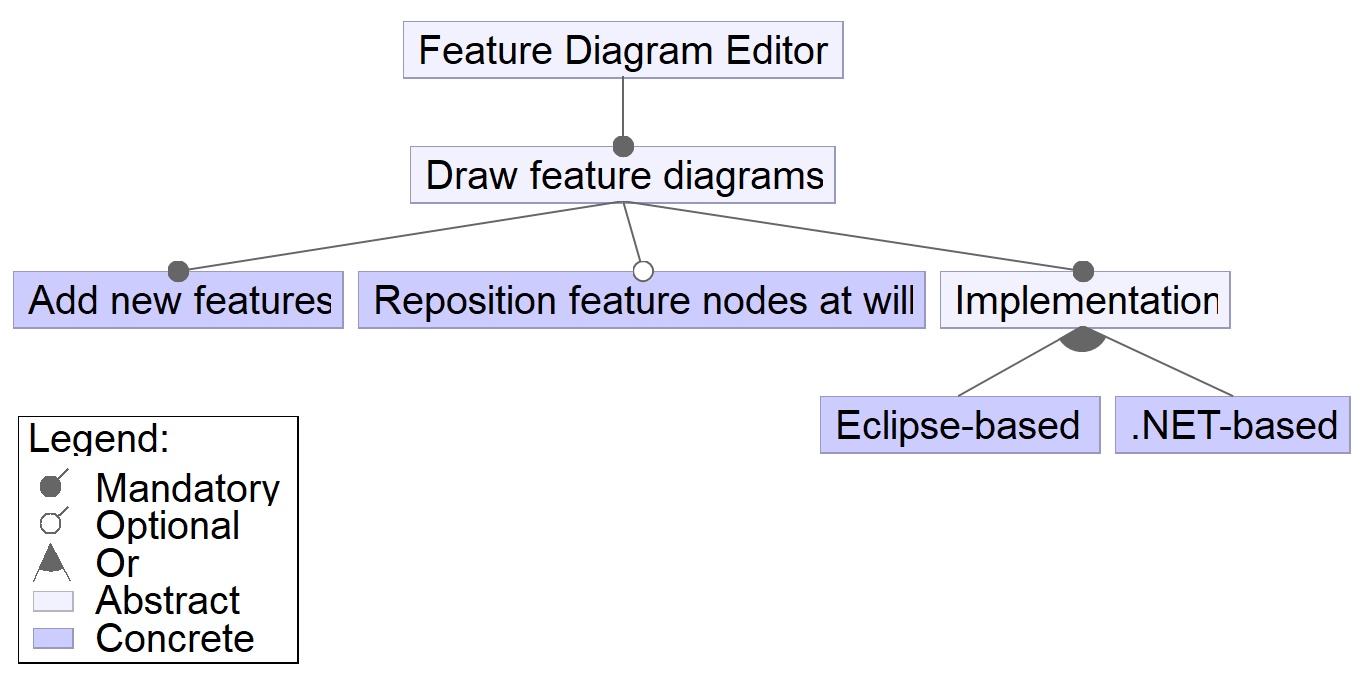
\includegraphics[width=0.7\textwidth]{featureDiagram.png}
\end{center}

Нотация очень простая --- характеристики бывают абстрактными (то есть теми, которые надо ещё декомпозировать перед тем как реализовать) и конкретными (пригодными к реализации), отношения между характеристиками бывают <<или>> (включающее и исключающее), обязательность и необязательность (то есть, без необязательной характеристики продукт вполне может существовать).

Для <<повседневного>> анализа требований диаграммы характеристик не очень удобны (отчасти потому, что их почти никто из редакторов не поддерживает, отчасти потому, что они получаются очень большими). Однако они активно используются в разработке линеек программных продуктов (например, если у вас есть Professional и Ultimate-версии, то можно отметить на общей диаграмме характеристик, какие характеристики куда попадают). Особенно хорошо это работает, если можно наладить автоматическую генерацию конфигурации продукта (или даже кода) по диаграммам.

Хороший пример такого подхода описан в статье D. Brugali et al., <<Variability Modeling of Service Robots Experiences and Challenges>> (2019) (точнее, у них про это целый проект BRICS, публикаций по нему много, эта даже не самая показательная, но одна из самых свежих). Товарищи занимаются конфигурированием ПО для сервисных роботов, что особенно сложно, потому что роботы имеют разную аппаратную конфигурацию, работают в разном окружении и предназначены для разных задач. Поэтому и программные платформы, и конкретное ПО приходится выбирать из массы вариантов и адаптировать под конкретного робота, задачи и даже аппаратная конфигурация которого может меняться по ходу дела.

Общая идея такая: описать все возможные характеристики аппаратной платформы, характеристики доступного ПО и получить диаграммы характеристик в духе:

\begin{center}
    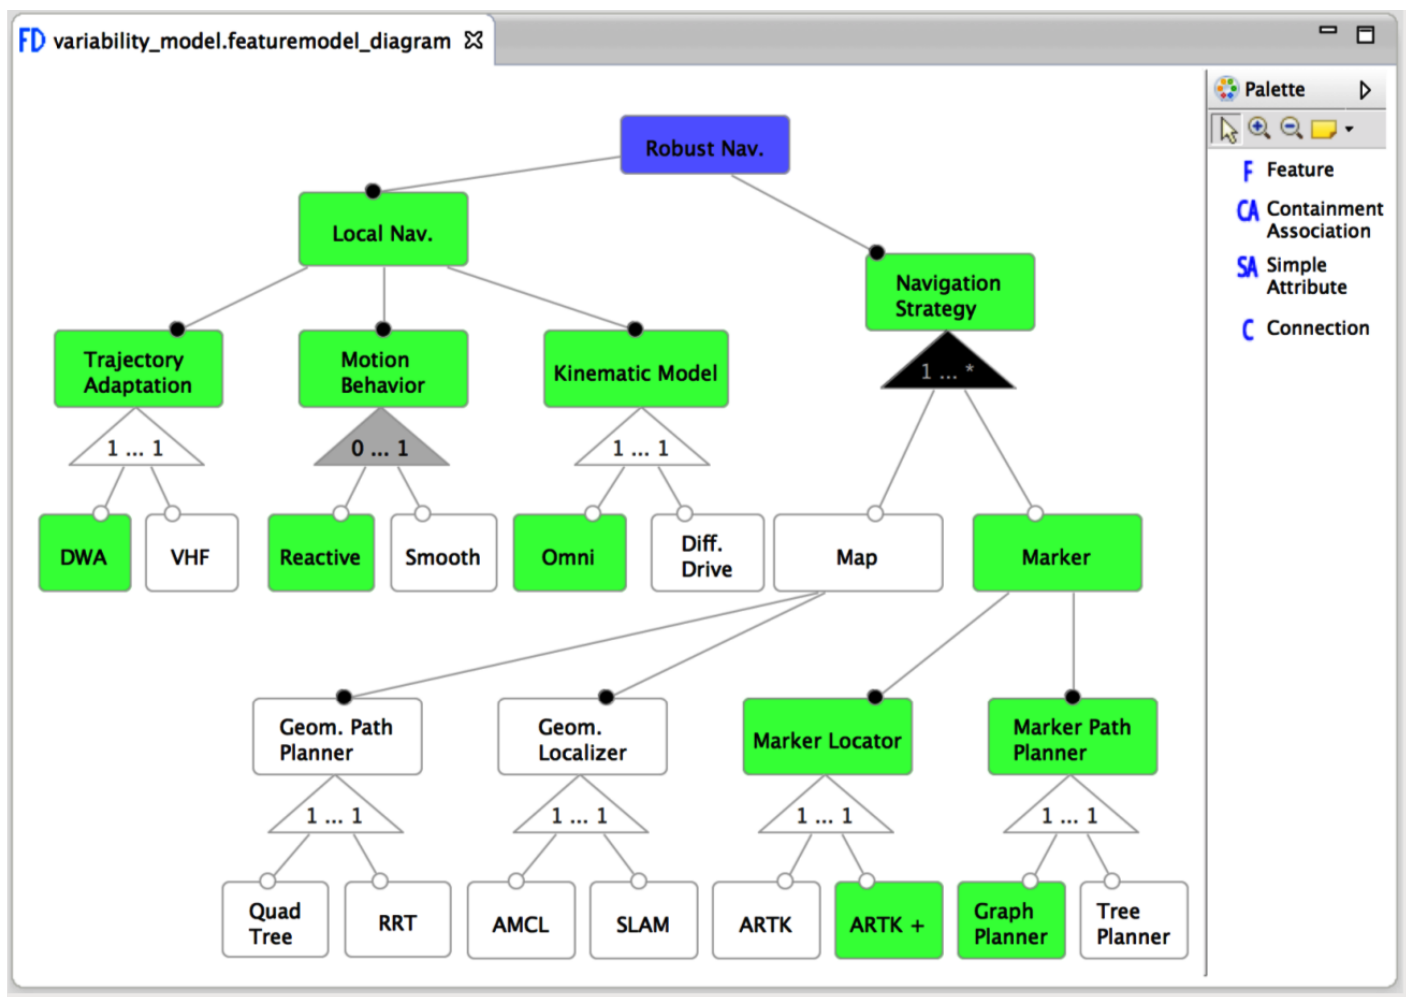
\includegraphics[width=0.9\textwidth]{featureDiagramExample.png}
    \attribution{D. Brugali et al.}
\end{center}

Дальше под конкретную задачу можно просто выбирать нужные характеристики, а система сама сгенерирует код, который развернёт на роботе нужный софт и правильно его сконфигурирует. На самом деле, там не всё так просто, есть ещё отображения между характеристиками аппаратной платформы и характеристиками ПО, зависимости между характеристиками (например, если на роботе нет камеры, то распознавать маркеры на стенах не выйдет), есть типовая архитектура, которая, собственно, позволяет конфигурировать систему, но это уже детали реализации и не относится к теме лекции.

\section{Feature tree}

Диаграммы характеристик довольно громоздки и их сложно рисовать, поэтому во время первоначального анализа требований (например, brainstorm-а по поводу нового проекта) можно использовать похожую, но более простую нотацию: дерево характеристик (feature tree, или их ещё называют fishbone diagram из-за внешней схожести со скелетом рыбы). Выглядят они так:

\begin{center}
    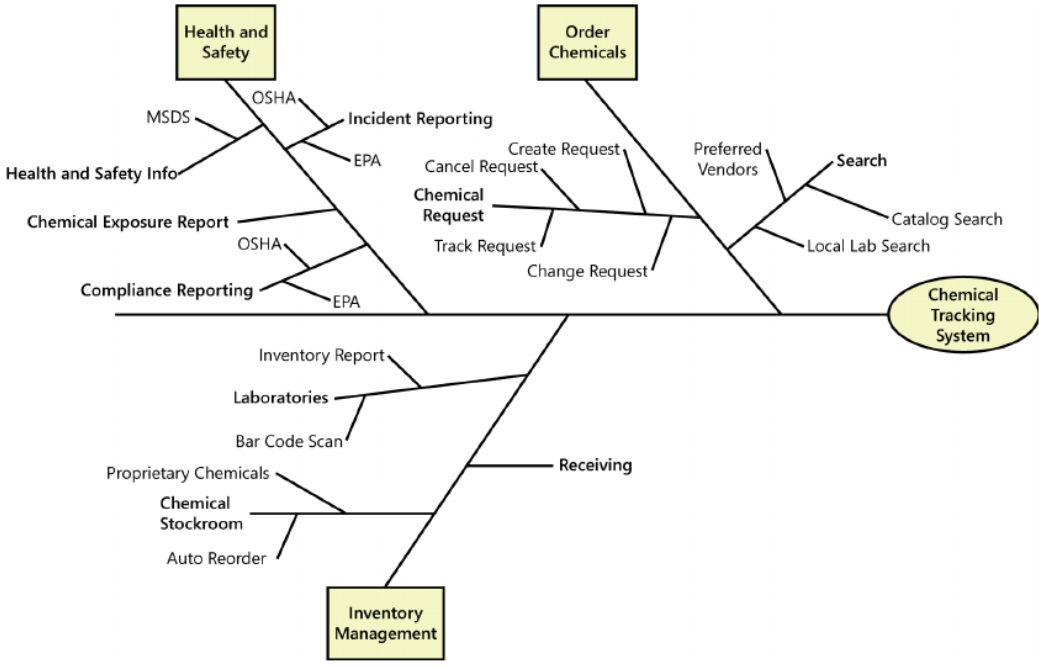
\includegraphics[width=0.7\textwidth]{featureTree.png}
\end{center}

<<Голова рыбы>> --- это система в целом, от неё отходит <<хребет>>, от которого отходят основные фичи. Они дальше детализируются более мелкими фичами, рисуемыми как ответвления от основных. На такой диаграмме никаких взаимосвязей не показать, но как инструмент первоначального анализа она может быть очень полезна. А потом уже можно нарисовать случаи использования, диаграмму характеристик и т.д.

\section{Диаграмма требований SysML}

Есть более формальная нотация дерева требований, в языке SysML. SysML изначально создавался как профиль (т.е. стандартное расширение) языка UML для моделирования больших систем, включавших в себя как программные, так и аппаратные компоненты, а так же людей и другие системы. Потом этот язык стал отдельным языком, туда добавили несколько новых видов диаграмм, в частности, диаграмма требований. Выглядит она так:

\begin{center}
    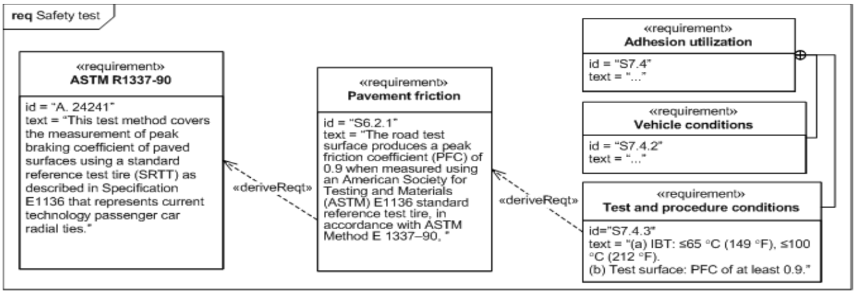
\includegraphics[width=0.8\textwidth]{sysMlRequirementDiagram.png}
    \attribution{OMG SysML 1.4 Specification}
\end{center}

Требования рисуются похоже на классы, со стереотипом \verb|<<requirement>>|, именем и идентификатором требования, и, главное, текстовым описанием. Требования могут находиться в разных отношениях (например, \verb|<<deriveReqt>>|, означающее, что одно требование является уточнением другого, или \verb|satisfy|, означающее, что какой-то элемент системы, например, класс, удовлетворяет или реализует то или иное требование).

Вот более содержательный пример:

\begin{center}
    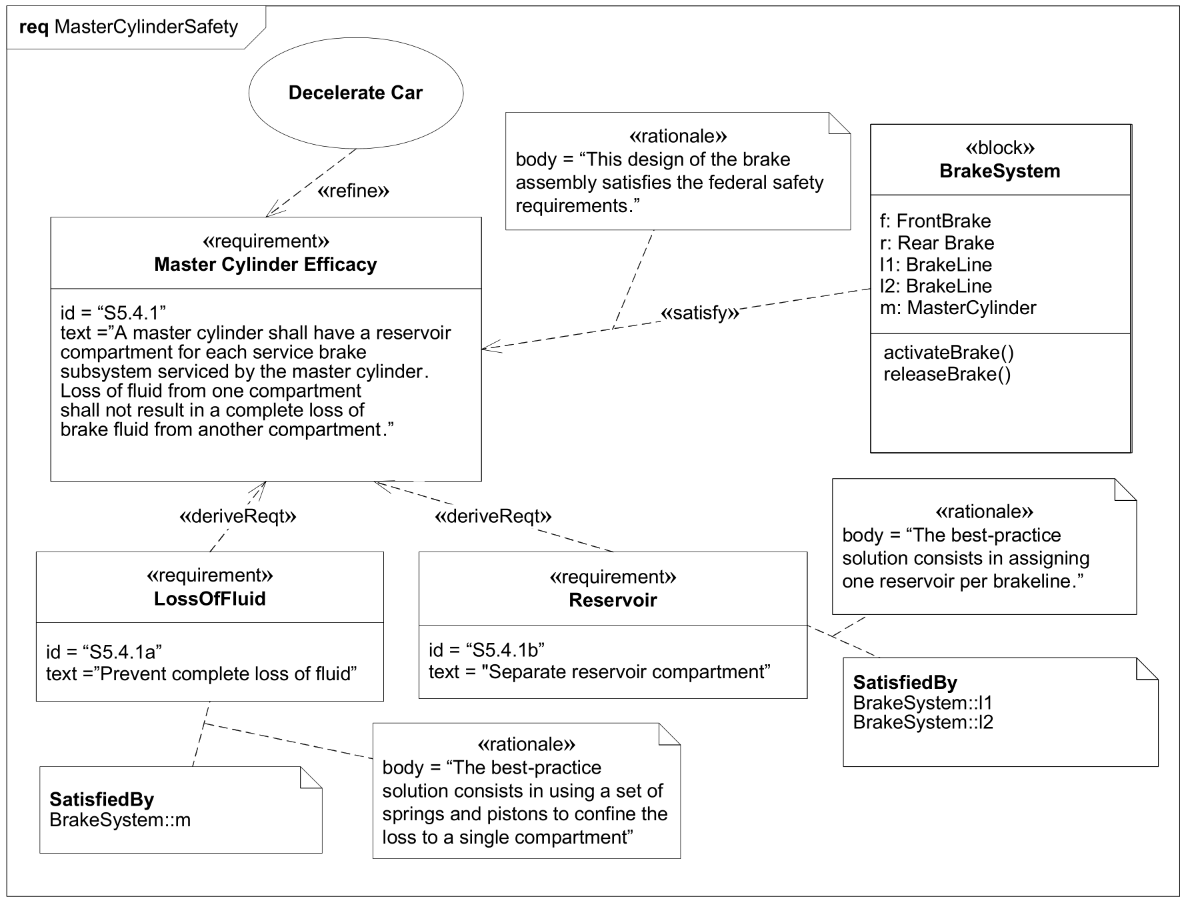
\includegraphics[width=0.7\textwidth]{sysMlRequirementsExample.png}
    \attribution{OMG SysML 1.4 Specification}
\end{center}

Как видим, на одной диаграмме могут рисоваться совершенно разные элементы. Случай использования <<Decelerate Car>> уточняется требованием <<Master Cylinder Efficacy>>, которое реализуется подсистемой <<BrakeSystem>> (классы и целые подсистемы в SysML называются блоками). При этом <<Master Cylinder Efficacy>> уточняется наличием требования на невозможность полной потери тормозной жидкости и наличием раздельных резервуаров тормозной жидкости для каждой из линий тормозной системы. Каждое требование поясняется комментарием \verb|<<rationale>>|, где написано, почему было принято такое решение.

Требования могут быть также уточнены сценарием тестирования (в SysML даже есть стандартные отношения \verb|<<verifies>>|/\verb|<<verifiedBy>>|). Сценарий тестирования может быть представлен в виде диаграммы активностей. Например, требования на работу тормозных колодок:

\begin{center}
    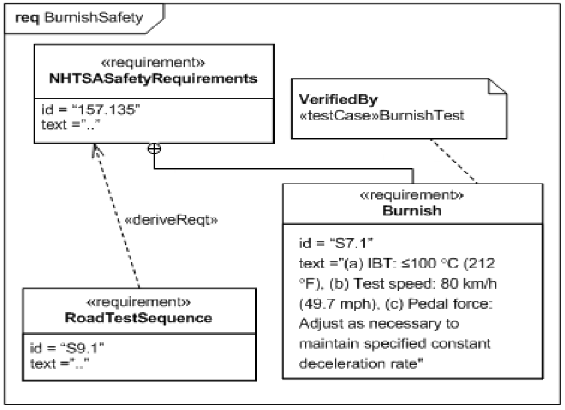
\includegraphics[width=0.5\textwidth]{sysMlRequirementsTest.png}
    \attribution{OMG SysML 1.4 Specification}
\end{center}

могут быть проверены следующим сценарием тестирования:

\begin{center}
    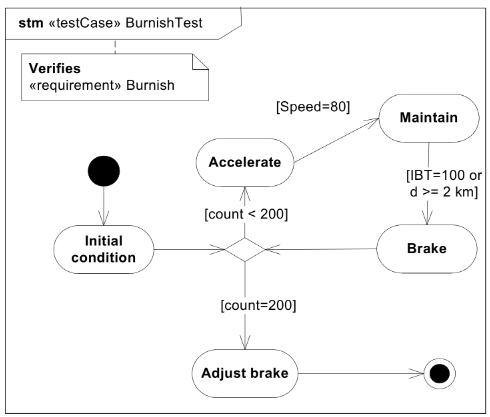
\includegraphics[width=0.5\textwidth]{sysMlRequirementsTestActivity.png}
    \attribution{OMG SysML 1.4 Specification}
\end{center}

\section{Диаграмма активностей UML}

Важной задачей на этапе анализа, помимо сбора требований, является ещё и анализ бизнес-процессов, которые (или часть которых) мы хотим автоматизировать. Для этого применяются несколько нотаций --- во-первых, диаграммы активностей UML, во-вторых, отдельный язык BPMN (Business Process Model and Notation), который, как и UML, состоит из нескольких видов диаграмм и специально предназначен для моделирования бизнес-процессов.

Но сначала про диаграммы активностей из UML, как более легковесный инструмент. Внешне они очень напоминают блок-схемы, но используются прежде всего не для моделирования алгоритмов (хотя и для этого тоже, иногда), а для моделирования поведения бизнес-процесса в целом. Кстати, термином <<бизнес-процесс>> в IT принято называть любой процесс работы в организации, может быть, и не связанный с бизнесом. Зачем вообще моделировать процессы --- во-первых, для того, чтобы понять, как в существующий процесс вписывается разрабатываемая система, во-вторых, это хороший способ визуализации сценария использования системы, с точки зрения пользователя.

Кстати, это одна из двух диаграмм UML, для которой описана семантика её исполнения, на основе сетей Петри. Вторая диаграмма --- это диаграмма конечных автоматов, про которую расскажут на лекциях попозже. Выглядит диаграмма активностей (также иногда встречается вариант перевода <<диаграмма деятельностей>>) так:

\begin{center}
    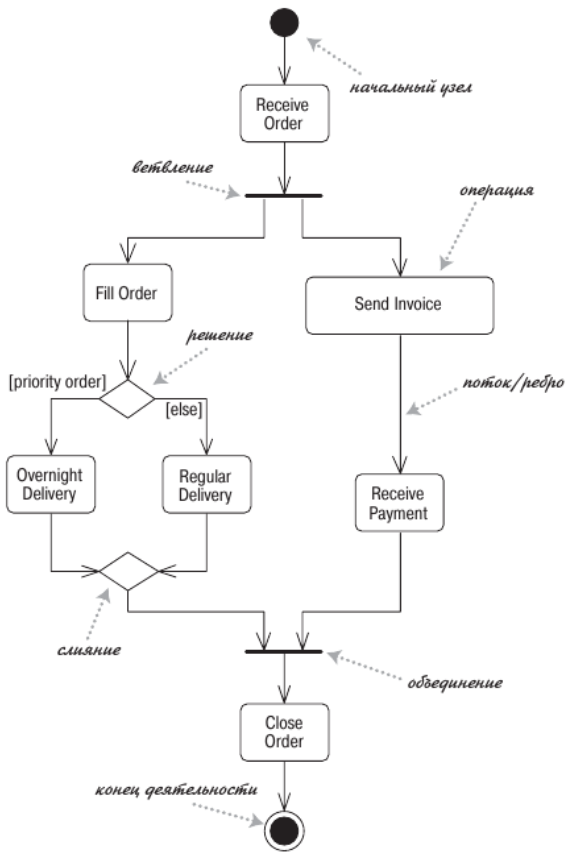
\includegraphics[width=0.5\textwidth]{activityDiagram.png}
    \attribution{М. Фаулер, UML. Основы}
\end{center}

<<Ветвление>>/<<объединение>> работает как fork/join для параллельных потоков --- <<ветвление>> разделяет исполнение на два или больше параллельных потоков, <<объединение>> ждёт, пока все входящие в него потоки закончат исполнение, и только после этого отдаёт управление дальше. Ничто не мешает потоки не объединять, тогда исполнение заканчивается, как только хотя бы один поток дойдёт до блока <<конец деятельности>>. По синтаксису каждый блок <<решение>> может иметь несколько веток (в этом смысле он похож на оператор switch/case в текстовых языках), но все ветки должны сходиться на блоке <<слияние>>. Причём, в отличие от блок-схем, условие пишется не в ромбике, а над каждой исходящей стрелкой, и условия должны быть взаимоисключающими.

Ещё на диаграмме активностей можно показать разделение работ по отделам организации или частям системы. Это важно в анализе бизнес-процессов, поскольку визуализирует разделение ответственности между частями организации. Рисуются разделы так:

\begin{center}
    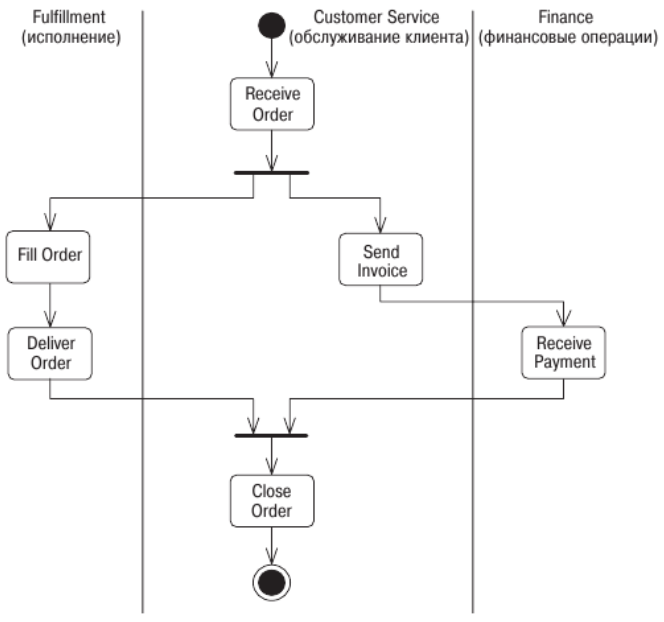
\includegraphics[width=0.5\textwidth]{activitySwimlanes.png}
    \attribution{М. Фаулер, UML. Основы}
\end{center}

А ещё, в отличие от блок-схем, есть возможность показать асинхронное взаимодействие с помощью сигналов. Рисуются они вот так:

\begin{center}
    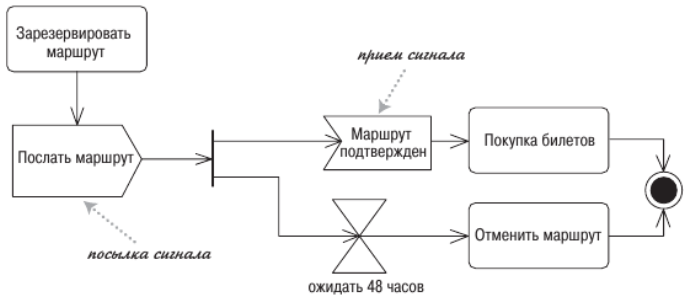
\includegraphics[width=0.6\textwidth]{activitySignals.png}
    \attribution{М. Фаулер, UML. Основы}
\end{center}

Сигналом чаще всего является отправка документа, но может быть и сетевой запрос, и электронное письмо, и что-то ещё, что отправляется за границы моделируемого бизнес-процесса. Блок <<посылка сигнала>> тут же возвращает управление и процесс продолжается вне зависимости от того, принял кто-то сигнал или нет. Блок <<приём сигнала>> ждёт указанный сигнал и продолжает процесс только когда сигнал поступит. Ещё есть блок <<таймер>>, который можно понимать как отложенный сигнал самим себе --- процесс ждёт указанное время, затем продолжается. На диаграмме выше показан типичный запрос с таймаутом.

\section{Business Process Model and Notation}

Для более продвинутого анализа бизнес-процессов используется отдельный язык BPMN (Business Process Model and Notation), который не входит в UML, хотя и является его близким родственником. Диаграммы активностей хороши, если у вас один-два бизнес-процесса с тремя-четырьмя участниками, однако в реальной жизни нередки ситуации, когда у организации более сотни субподрядчиков, и взаимодействие с каждым --- отдельный бизнес-процесс, а работа организации --- это тоже бизнес-процесс, включающий в себя эти бизнес-процессы. Если вдруг не повезло автоматизировать бизнес-процессы такого масштаба, то без BPMN не обойтись. Правда, в этом случае не стоит доверять анализ бизнес-процессов архитектору, лучше нанять отдельного бизнес-аналитика. Поэтому BPMN несколько реже встречается в программистской практике, чем диаграммы активностей UML, и поэтому в этом курсе про BPMN будет существенно меньше, чем могло бы быть, но поскольку архитектору надо как-то общаться с аналитиками и вообще знать, что такое бывает, про BPMN всё-таки будет.

Стандарт BPMN 1.0 был принят в 2004 году, как раз примерно в те времена, что и UML 2.0, тем же консорциумом Object Management Group, который управляет UML. BPMN также определён с помощью метамодели и стандарты очень похожи по принципам определения языка, но BPMN, тем не менее, отдельный язык (точнее, как и UML, набор языков).

BPMN можно воспринимать как сильно продвинутые диаграммы активностей. Он позволяет, в частности, визуализировать взаимодействие нескольких процессов (в отличие от диаграмм активностей, где посылка и приём сигналов просто не связанные между собой блоки, в BPMN рисуются нормальные стрелочки), имеет гораздо больший набор блоков-ветвлений (в том числе и с параллельными потоками), блоков ожидания разных событий, качественную поддержку исключений. Так же, как и диаграммы активностей, BPMN имеет исполнимую семантику, но, в отличие от диаграмм активностей, эта семантика может быть использована для реального исполнения бизнес-процесса в информационной системе --- благодаря стандартизованным правилам преобразования диаграмм на BPMN в XML-документы на BPEL (Business Process Execution Language), настоящем исполнимом языке описания бизнес-процессов, который поддерживают многие движки-исполнители\footnote{см. \url{https://en.wikipedia.org/wiki/List_of_BPEL_engines}}.

\subsection{Диаграмма процессов}

Вот так выглядит самая, пожалуй, известная диаграмма BPMN (которую часто путают с BPMN вообще, например, в википедии) --- диаграмма процессов (process diagram):

\begin{center}
    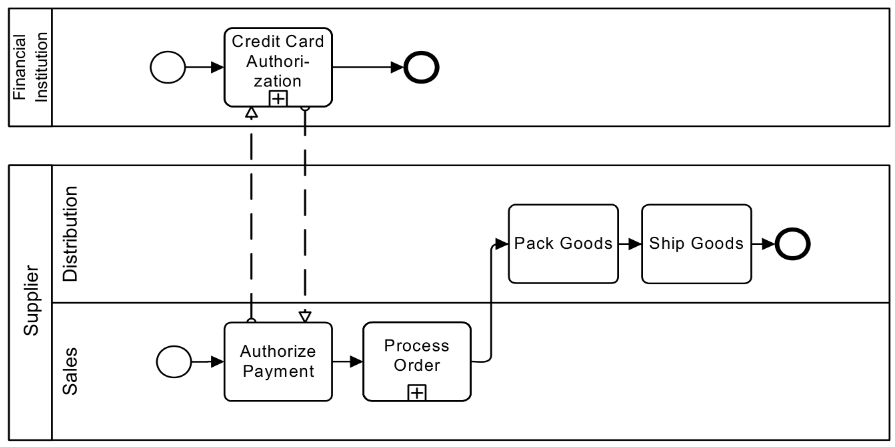
\includegraphics[width=0.9\textwidth]{bpmnExample.png}
    \attribution{OMG BPMN 2.0 Specification}
\end{center}

Тут изображены два бизнес-процесса двух независимых организаций, общающихся посылкой и приёмом сообщений. Бизнес-процесс одной из огранизаций поделен на два раздела, но тем не менее, это один бизнес-процесс, на что указывает единый поток управления. Плюсик внутри активности означает, что активность раскрывается в другой, более детализированный бизнес-процесс. Пользоваться такими диаграммами можно как диаграммами активностей UML, а подробнее прочитать про их синтаксис можно, как ни странно, в русской википедии (\url{https://ru.wikipedia.org/wiki/BPMN}), если не хотите ознакомиться с почти шестисотстраничным стандартом\footnote{\url{https://www.omg.org/spec/BPMN/2.0/}}. Вот табличка с видами событий оттуда:

\begin{center}
    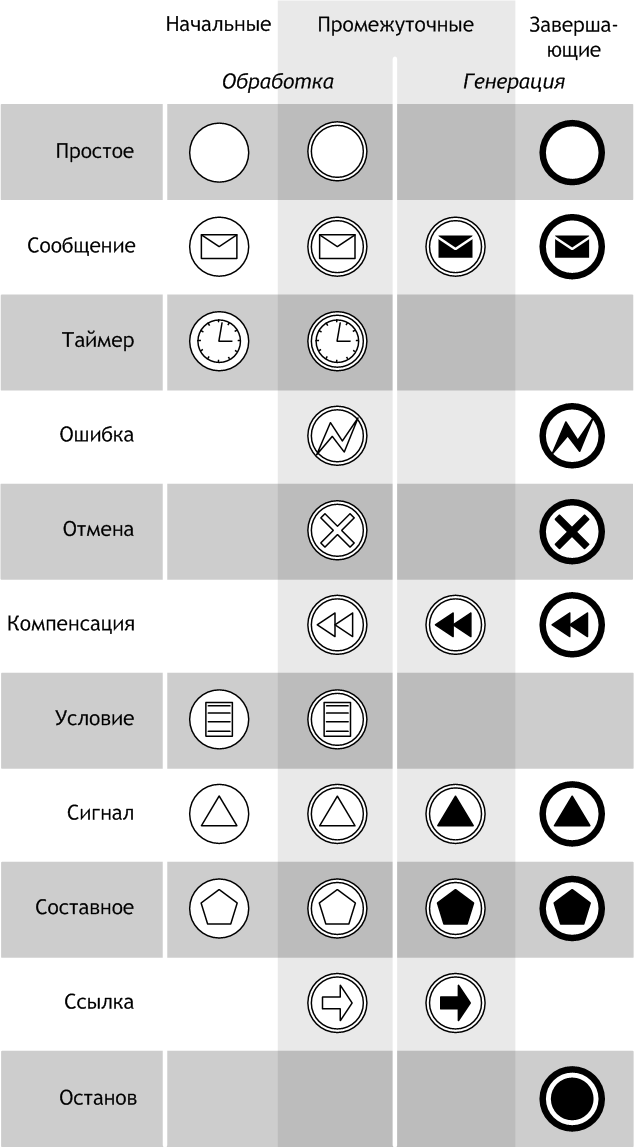
\includegraphics[width=0.4\textwidth]{bpmnEvents.png}
    \attribution{\url{https://ru.wikipedia.org/wiki/BPMN}}
\end{center}

Пояснять тут её нет смысла, потому что в википедии всё подробно описано, но представление о том, что в BPMN бывает и почему BPMN лучше для анализа сложных процессов, чем диаграмма активностей UML, это даёт. А вот несколько менее эпичная таблица с типами логических операторов (опять же, из википедии, и, опять же, без пояснений):

\begin{center}
    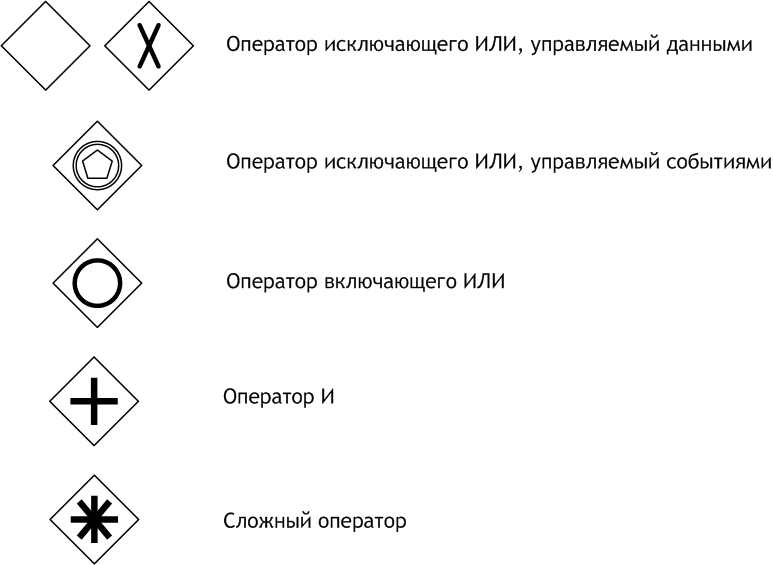
\includegraphics[width=0.5\textwidth]{bpmnGateways.png}
    \attribution{\url{https://ru.wikipedia.org/wiki/BPMN}}
\end{center}

\subsection{Диаграмма хореографии}

Второй вид диаграмм BPMN --- диаграмма хореографии (choreography diagram) --- описывает исключительно взаимодействие между бизнес-процессами. На ней не рисуется кто что должен делать, на ней рисуется, кто когда с кем должен общаться. Выглядит это так:

\begin{center}
    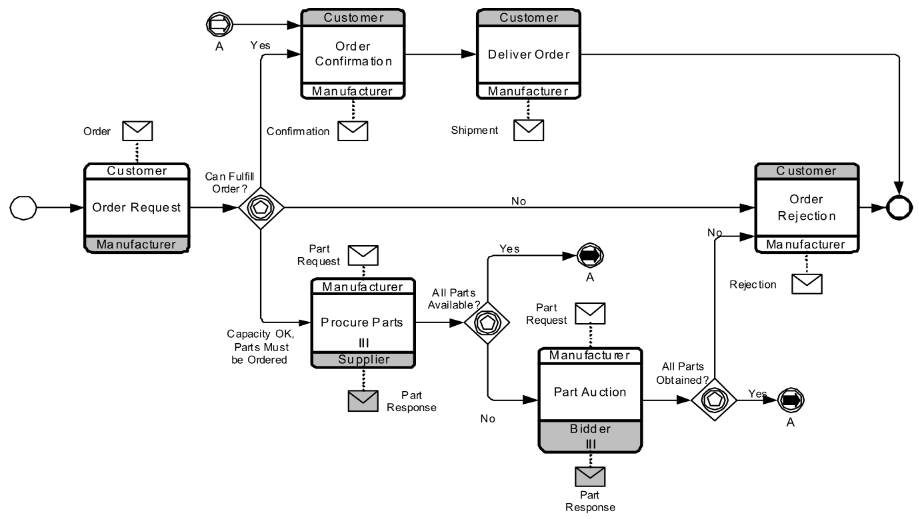
\includegraphics[width=0.9\textwidth]{bpmnChoreography.png}
    \attribution{OMG BPMN 2.0 Specification}
\end{center}

Прямоугольники со скруглёнными углами --- это точки общения между процессами, белым цветом выделен инициатор взаимодействия, серым --- тот, кто должен ему ответить, конвертиком --- сообщение или документ. Как видим, ветвления и события тут рисуются, а активности --- нет. Такая диаграмма нужна, если попытка изобразить процессы в дорожках на диаграмме процессов привела бы к хаосу из стрелочек.

\subsection{Диаграмма диалогов}

И последняя диаграмма BPMN --- диаграмма диалогов (conversation diagram), она показывает схему общения бизнес-процессов, не в смысле когда кто с кем общается, как диаграмма хореографии, а в смысле кто с кем в принципе может общаться. Выглядит диаграмма вот так:

\begin{center}
    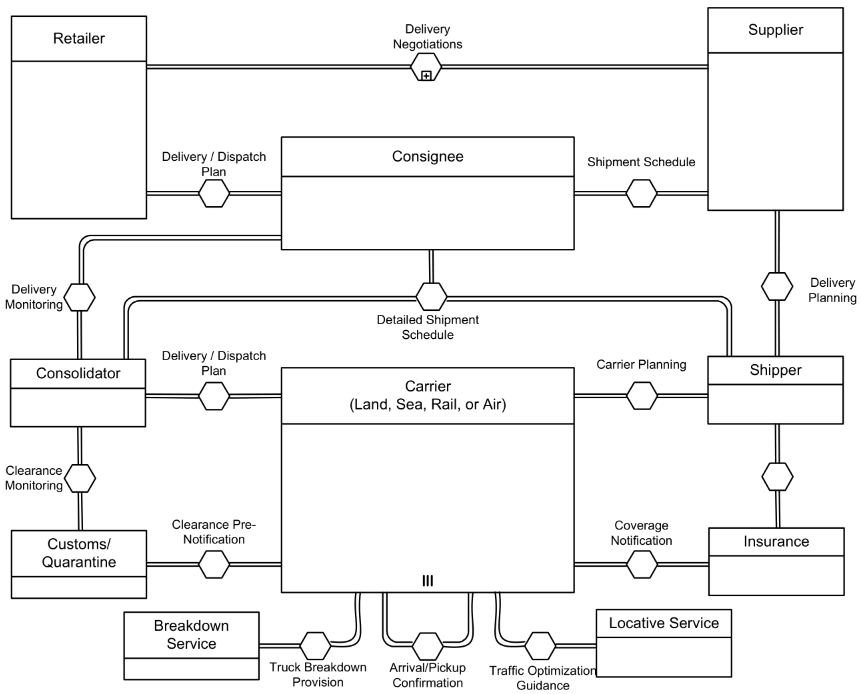
\includegraphics[width=0.9\textwidth]{bpmnConversation.png}
    \attribution{OMG BPMN 2.0 Specification}
\end{center}

Прямоугольниками показаны участники взаимодействия, двойными линиями с шестиугольниками --- общение между участниками. Плюсик внутри шестиугольника показывает, что взаимодействий между участниками много и они могут быть уточнены диаграммами хореографий или диаграммами процессов без деталей (это когда просто рисуются дорожки и сообщения, без внутреннего содержимого, так тоже можно). Три вертикальные черты внутри участника взаимодействия означают, что участников на самом деле может быть много.

На этом закончим обзор BPMN (очень-очень краткий, там ещё куча разных тонкостей, про которые надо знать, чтобы стать нормальным аналитиком, но у нас тут курс по архитектуре). Можно дополнительно ознакомиться с примерами BPMN-диаграмм из небольшого, неформального, но очень полезного документа от OMG: \url{https://www.omg.org/cgi-bin/doc?dtc/10-06-02}

\section{Задача на остаток пары}

Для того, чтобы попрактиковаться в анализе требований и рисовании разных диаграмм, предлагается проанализировать запрос на разработку ПО из реальной практики. В командах по два человека нужно проанализировать запрос \url{https://bit.ly/defects-rfp} и построить по нему:

\begin{enumerate}
    \item диаграмму случаев использования, описывающую пользователей и случаи использования разрабатываемого приложения;
    \item диаграмму активностей для основного бизнес-процесса, поддерживаемого приложением --- регистрации и ремонта дефекта;
    \item BPMN-диаграмму для всего бизнес-процесса завода, включая внешних его участников.
\end{enumerate}

Сдавать нужно в свои репозитории отдельным пуллреквестом, либо исходник диаграммы, либо .md-файл со ссылкой на проект в какой-либо облачной рисовалке (в этом случае не забудьте расшарить). И не забудьте указать, с кем вы в команде.

\end{document}
